
\medskip

Une famille désire acheter, pour les enfants, une piscine cylindrique hors sol équipée d'une pompe électrique. Elle compte l'utiliser cet été du mois de juin au mois de septembre inclus. Elle dispose d'un budget de $200$~\euro.

À l'aide des documents suivants, dire si le budget de cette famille est suffisant pour l'achat de cette piscine et les frais de fonctionnement.

\emph{Laisser toute trace de recherche, même si elle n'est pas aboutie.}

\medskip

\begin{tabularx}{\linewidth}{|X|m{5.8cm}|}\hline
\textbf{Document 1}

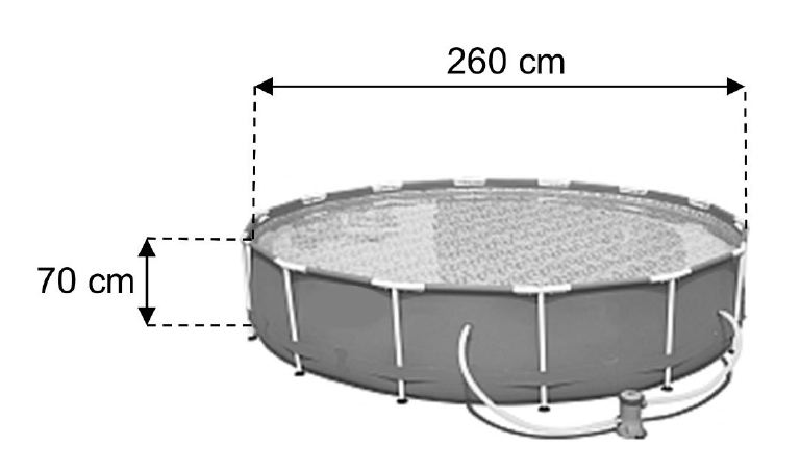
\includegraphics[width=6cm]{piscine_CE_2019}

\medskip

\textbf{Caractéristiques techniques :}

$\bullet~$ Hauteur de l'eau : $65$ cm

$\bullet~$Consommation électrique moyenne de la pompe :
$3,42$ kWh par jour.

$\bullet~$ Prix (piscine + pompe) : $80$~\euro.&\begin{tabular}{m{5.6cm}}\hline

\textbf{Document 2}\\

Prix d'un kWh: 0,15~\euro.\\

Le kWh (kilowatt-heure) est l'unité de mesure de l'énergie électrique.\\ \hline
\textbf{Document 3}\\

Prix d'un m$^3$ d'eau : $2,03$~\euro.\\ \hline
\textbf{Document 4}\\

Le volume d'un cylindre est donné par la formule suivante:\\

\[V = \pi \times  r^2 \times h\]

où $r$ est le rayon du cylindre et $h$ sa hauteur.\\ 
\end{tabular}\\ \hline
\end{tabularx}


